\documentclass{fisatproject}
\title{Hologram with Haptic Feedback}
\team{Leo Varghese \\ Mohit Rajan E\\ Ria Alexander}
\author{Mohit Rajan E}
\begin{document}
\maketitle
\makecert

\newpage
\pagenumbering{roman}
\setcounter{page}{1}
\newgeometry{top=4cm,bottom=0.1cm}
\thispagestyle{plain}
\renewcommand\abstractname{ABSTRACT}
\begin{abstract}
\vspace{5cm}
This paper is intended to analyze and discuss the developments made so far in the field of holography and holographic projection, it discusses the feasibility and the possibilities in the area of touchable holograms, which can be interacted using hand gestures. In this paper, first we will discuss some rudimentary matters about what a hologram is and a short description of how they are created. Then we will move on to how we can make a hologram move as per our hand gestures and provide haptic feedback. In this paper the focus is on the feasibility study of some methods and the analysis and consequences of these methods. We will see some challenges in the whole process and then some discussion about future scopes of this technology and where this technology can lead us.
\end{abstract}



\newpage
\renewcommand\abstractname{Contribution by Author}
\thispagestyle{plain}
\begin{abstract}
\vspace{5cm}
Author Contribution  Goes Here
\vspace{1cm}
\begin{flushright}
Student Name
\end{flushright}
\end{abstract}

\newpage
\renewcommand\abstractname{ACKNOWLEDGMENT}
\thispagestyle{plain}
\begin{abstract}
\vspace{5cm}
Your Acknowledgement Goes Here
\vspace{1cm}
\begin{flushright}
Student 1
\end{flushright}
\end{abstract}
\newpage

\restoregeometry
\tableofcontents
\newpage

\cleardoublepage
\addcontentsline{toc}{chapter}{\listfigurename}
\listoffigures
\newpage

\cleardoublepage
\addcontentsline{toc}{chapter}{\listtablename}
\listoftables
\newpage



\chapter{Introduction}
\pagenumbering{arabic}
\setcounter{page}{1}
\renewcommand{\baselinestretch}{1.50}
\section{Overview}
The mathematical roots of the idea of fractals have been traced through a formal path of published works, starting in the 17th century with notions of recursion, then moving through increasingly rigorous mathematical treatment of the concept to the study of continuous but not differentiable functions in the 19th century, and on to the coining of the word fractal in the 20th century with a subsequent burgeoning of interest in fractals and computer-based modelling in the 21st century.
\begin{figure}[h!]
\begin{center}
\includegraphics[scale=.2]{mandelbrot}
\caption{Mandelbrot Fractal}
\end{center}
\end{figure}
The word "fractal" often has different connotations for laypeople than mathematicians, where the layperson is more likely to be familiar with fractal art than a mathematical conception. The mathematical concept is difficult to formally define even for mathematicians, but key features can be understood with little mathematical background.

The feature of "self-similarity", for instance, is easily understood by analogy to zooming in with a lens or other device that zooms in on digital images to uncover finer, previously invisible, new structure. If this is done on fractals, however, no new detail appears; nothing changes and the same pattern repeats over and over, or for some fractals, nearly the same pattern reappears over and over. Self-similarity itself is not necessarily counter-intuitive (e.g., people have pondered self-similarity informally such as in the infinite regress in parallel mirrors or the homunculus, the little man inside the head of the little man inside the head...). 

Lorem ipsum dolor sit amet, consectetur adipiscing elit. Morbi urna mauris, sagittis sit amet aliquet ut, facilisis et nibh. Praesent turpis tortor, dignissim ut interdum eu, porttitor ut orci. Curabitur laoreet malesuada fermentum. In posuere, purus eu pulvinar luctus, eros urna tempor magna, eu tincidunt erat eros nec turpis. Vestibulum at semper lacus. Nullam tristique lacus vel nibh porta a vehicula tellus volutpat. Pellentesque cursus ullamcorper ante, ut eleifend nisl aliquam id. Nulla porta ornare fermentum. Aliquam id magna sed erat malesuada viverra. Donec non mauris eros, nec egestas ligula. Suspendisse eu tempor ligula. Aliquam egestas nulla vel augue iaculis iaculis nec in risus. Pellentesque habitant morbi tristique senectus et netus et malesuada fames ac turpis egestas. Praesent malesuada fringilla sapien a faucibus.

\section{Problem Statement}

\par In the current education system students are taught to learn formulas and how to use them but not to reason or understand the logic behind them, causing then to forget it in a short peroid.It is a typical longitudianl learning approah. Our brain system is not just longitudianl in learning process, but much more complex. Current education system evolved on the basis of visual and audotory senses and their application leads to memmorizing the content of learning rather than creaing a holistic perceprtion.
% which can be based on the enormous untapped abilities of the human brain.
It is observed that the current education system  uses mainly audio methods to teach students.
In India around 10\% of students suffer from some form of learning disibility[1]. Research also point to the fact that visual working memory is better in students with learning disibility rather than audority working memory[2].
It can be infered that a modern method of learning should be devloped in order to increase the efficiency of learning process.

\par To addres this issue  we propose a system which uses a hologramic display with haptic feedback by the interaction of using hand gestures. This project will focus on developing a system as described above to introduce a new approch to learn basic geometry.

\section{Objective}

To create a system which also includes somesthetic senses to learning. To achive this a hologramic display with haptic feedback is proposed. The proposed system can be used to project objects in mid-air which can be intracted by using the hand gestures to view new objects, change or modifiy its properties like size, view etc.

\chapter{Literature Review}

The world population is the sum of all humans on Earth. As of today, it is estimated to number 7.004 billion by the United States Census Bureau. The USCB estimates that the world population exceeded 7 billion on March 12, 2012. According to a separate estimate by the United Nations Population Fund, it reached this milestone on October 31, 2011.
\begin{table}[h!]
\begin{center}
\begin{tabular}{|c|c|c|c|}
\hline Rank & Country & Population  & Percentage  \\ 
\hline 1 & China & 1,347,350,000 & 19.24\% \\ 
\hline 2 & India & 1,210,193,422  & 17.28\% \\ 
\hline 3 & United States & 313,269,000 & 4.47\% \\ 
\hline 
\end{tabular}
\caption{World Population Table} 
\end{center}
\end{table}
The world's population is unevenly distributed, with six of Earth's seven continents being permanently inhabited on a large scale. As of 2012, Asia is the most populous continent, with its 4.1 billion inhabitants accounting for over 60\% of the world population. The world's two most-populated countries alone, China and India, constitute about 37\% of the world's population. Africa is the second-most-populated continent, with around 1 billion people, or 15\% of the world's population. Europe's 733 million people make up 11\% of the world's population, while the Latin American and Caribbean regions are home to 589 million (9\%).


\chapter{Design}

The proposed system consist of three sub-systems
\begin{itemize}
    \item  Display
    \item Haptic feedback
    \item Hand gesture regonazing system.
    \item Software compontent ? (is this required?)
\end{itemize}
\subsection{Display}
Hologram was selected as the method of display. Since previous  research has shown learning gemotry with hologram is better than tradional methods[3].

\subsection{Haptic feedback}
Haptic feedback is added to add a somesthetic senses to learning. And also as a response to convay the previous commanf by the user has been registred.

\subsection{Hand Gesture}
Hand Gestures are used as the input to the system and will be used by the user to intract with the system.
{Required bellow part?}
The hand geuster is proccess using Google  MediaPipe libaray.

\section{Proposal}
In mathematics, Stirling's approximation (or Stirling's formula) is an approximation for large factorials. It is named after James Stirling.

The formula as typically used in applications is:

$$
\ln (n!) = n \ln n - n  + O(\ln(n))
$$

\chapter{Work Plan}
Our work plan have different phases .
 Our work will progress through these phases.
 \begin{itemize}
     \item Holographic projection
     \item Ultrasonic phased array for tactile feedback.
     \item Hand Gesture recognition
 \end{itemize}
 \subsection{Holographic Projection}
    The first step of our work is to make holographic projection of our an input image.
    There are different methods to achieve this.
    \begin{itemize}
        \item Thin Amplitude Hologram
        \item Thin Phase Holograms
        \item Volume Hologram
        \item Reflection Hologram
    \end{itemize}
    The decision to choose a method depends upon the efficiency of the display.
 \subsection{Tactile feedback}
    In this phase, An array of ultrasonic sensors are used to provide tactile feedback.
    Phased array creates adisturbance in the air that the user can feel whenthey pass their fingertips across it.
    \begin{figure}[h!]
        \begin{center}
        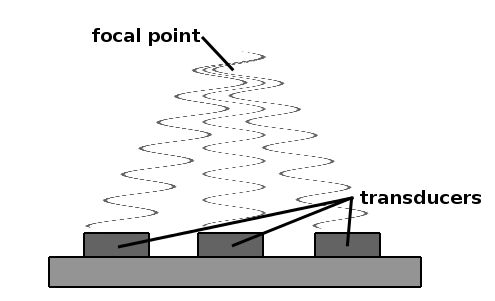
\includegraphics[scale=.8]{images/img1.jpg}
        \caption{Tactile Feedback}
        \end{center}
        \end{figure}
 \subsection{Hand Gesture recognition}
     For hand gesture recognition, Machine learning techniques are used.
     Different hand sign are trained using a machine learning model.
     A model is selected selected based on the accuracy of the model.
     The live image of hand is captured using a camera and detected using machine learning.
     Based on the sign, The image is classifed and the change is reflected real-time.
 \section{Budget}


\chapter{Conclusion}

An intrusion detection system (IDS) \cite{nist} is a device or software application that monitors network and/or system activities for malicious activities or policy violations and produces reports to a Management Station.


Donald Ervin Knuth \cite{knuth} is a computer scientist and Professor Emeritus at Stanford University. He is the author of the seminal multi-volume work The Art of Computer Programming. Knuth has been called the "father" of the analysis of algorithms


\begin{thebibliography}{1}
\bibitem{nist} K. Scarfone and P. Mell, ``Guide to intrusion detection and prevention systems
(idps),'' \textit{NIST Special Publication}, vol. 800, no. 2007, p. 94, 2007.
\bibitem{knuth} Wikipedia, ``Donald knuth.'' \url{http://en.wikipedia.org/wiki/Donald_Knuth}.


\end{thebibliography}
\end{document}
